\documentclass[]{article}

%opening

\usepackage{amsmath}
\usepackage{amsfonts}
\usepackage{float}
\usepackage{hyperref}
\usepackage[explicit]{titlesec}
\usepackage{xcolor}
\usepackage{graphicx}
\usepackage{indentfirst}

\title{Final Report}
\author{
	Nikolay Pavlenko\\
	\texttt{n.pavlenko@innopolis.university}
}
\begin{document}
	\maketitle
	\section{Introduction}
	While searching for the possible ways to organize a movie recommendation system , I have decided to implement a Graph Neural Network. In this approach, each movie and user can be represented as nodes in a graph, and the interactions or relationships between them can be modeled as edges. Movie-user interactions, such as ratings, can be incorporated into the graph structure as edge values. A GNN could then be employed to learn node embeddings, capturing both the features of movies and users and their complex relationships. This enables the model to make personalized recommendations by leveraging the graph structure and learning latent representations that encode user preferences and movie characteristics. Additionally, GNNs inherently handle collaborative filtering by considering the connections between users who have similar preferences. This approach allows for a more dynamic and context-aware recommendation system that can adapt to the evolving interactions within the movie-user graph. \\
	
	After searching for an implementation of a GNN fit for a movie recommendations system, I have decided to use \cite{main} as the model that would be train on the given dataset, as, unlike many other implementations I have seen, it also leverages movie genre in its predictions, rather than disregarding them and focusing solely on relationships between encoded users ans movies. 
	\\
	\section{Data Exploration}
	Before moving forward with the selection of a model for detoxification, I had to analyse and modify the data before feeding it to the model. The dataset used was MovieLens 100K. In my solution I have used two primary files as dataset sources:
	\begin{enumerate}
		\item \textbf{u.data} - full dataset of 100000 ratings by 943 users on 1682 items. Users and items are numbered consecutively from 1. The data is randomly ordered. To prepare this dataset for the model I have converted the id columns to categorical from float, and ensured that there had been no nulls in the dataset.
		\item \textbf{u.item} - information about the items (movies). This is a tab separated list of movie id, movie title, release date, video release date, IMDB URL, and genres. The last 19 fields are genres and contain binary values. \\
		When searching for null values, I have found that this dataset had a lot of them in the information on the video release date, so it was dropped. IMDB URL also probably had no influence on the desire of a person to watch a movie, so it was dropped as well. The only remaining null in the release date of a placeholder for an unknown movie was filled with the earliest date available in the dataset. \\
	\end{enumerate}
	
	\section{Solution Implementation}
	This dataset contained a lot of information on the movie genres - in order to use them in the model predictions I had to take a few steps to modify them: 
	\begin{enumerate}
		\item I iterated over each row in the dataframe, and for each row, I constructed a string of genres based on the binary values in the \textbf{genre\_id} column. My idea was to create a string that represents the genres associated with each movie, where genres are separated by the '|' character.
		\item Then I used the CountVectorizer from scikit-learn (used to convert a collection of text data into a bag-of-words representation) to transform the created genre strings into a binary matrix \textbf{genres\_encoded}. This matrix encoded the presence or absence of each genre for each movie.
	\end{enumerate}.
	
	After finalizing the pre-processing work on the original datasets, I was able to define a custom dataset from those two, which was then used in the training and evaluation of the model (80/20 train/test split). \\
	It initializes with user-item interaction data and additional movie information, including encoded genres. The class extracts movie, user, and rating information from the datasets and converts textual movie genres into a tensor of genre indices. It ensures that the genre tensor length does not exceed a specified maximum count. The dataset was created to be used within PyTorch's DataLoader framework for efficient training and evaluation of movie recommendation models, encapsulating the necessary data processing steps for neural network input. The class also includes a check to ensure valid user IDs within a specified range. \\
	
	The model used in my solution is MovieLensNet. Its structure can be described in the following way:
	\begin{enumerate}
		\item \textbf{Embedding Layers}:
		\begin{itemize}
			\item \textbf{Movie Embedding}: Utilizes an Embedding layer to transform movie IDs into dense vectors of fixed size (embedding\_size). This enables the model to capture latent features associated with each movie.
			\item \textbf{User Embedding}: Similar to the movie embedding, this layer transforms user IDs into dense vectors, facilitating the capture of latent user features.
		\end{itemize}
		\item \textbf{Graph Convolutional Layers}:
		\begin{itemize}
			\item \textbf{Concatenation of Movie and User Embeddings}: The embeddings from the movie and user are concatenated to form a feature vector, representing the nodes in the graph. The goal is to capture the relationships between movies and users in a unified representation.
			\item \textbf{Genre Embedding}: Inclusion of genre information is crucial for enhancing the graph's structural understanding. The genre information is embedded using a Linear layer, creating embeddings for each genre.
		\end{itemize}
		\item \textbf{Fully Connected (Linear) Layers}:
		\begin{itemize}
			\item \textbf{FC1 (Fully Connected Layer 1)}: Accepts the concatenated embeddings and genre information. This layer applies a linear transformation to the input, transforming it to a hidden representation (hidden\_dim). Activation is performed using Rectified Linear Unit (ReLU), introducing non-linearity.
			\item \textbf{FC2 (Fully Connected Layer 2)}: Further applies a linear transformation and ReLU activation, capturing higher-level abstractions in the data.
			\item \textbf{FC3 (Fully Connected Layer 3)}: The final fully connected layer produces a single output, representing the predicted rating for a given movie-user pair.
		\end{itemize}
		\item \textbf{Flattening and Processing}:
		\begin{itemize}
			\item \textbf{Flattening}: Before entering the fully connected layers, the concatenated feature vector is flattened to ensure compatibility with the linear layers.
			\item \textbf{ReLU Activation}: Applied after each linear layer, introducing non-linearity and enabling the model to learn complex patterns.
		\end{itemize}
	\end{enumerate}
	
	\section{Training Process}
	
	\begin{enumerate}
		\item \textbf{Hyperparameters}: 
		\begin{itemize}
			\item \textbf{embedding\_dim} - size of the embedding vectors for movies and users, equal to 16
			\item \textbf{number\_epochs} - total number of training epochs, equal to 10
			\item \textbf{hidden\_dim} - dimensionality of the hidden layers in the fully connected part of the model, equal to 32
			\item \textbf{dropout\_p} - probability of dropout, which is a regularization technique to prevent overfitting, equal to 0.5
		\end{itemize}
		\item \textbf{Model Initialization}: MovieLensNet model is instantiated with the specified hyperparameters. This model is designed for collaborative filtering, taking into account movie and user embeddings along with genre information.
		\item \textbf{Training Setup}: The number of training samples is determined by the length of the training DataLoader (num\_train\_samples). The Mean Squared Error (MSE) loss (criterion) and Adam optimizer (optimizer) are defined.
		\item \textbf{Training Loop}: The training loop runs for the specified number of epochs.
		Inside each epoch, the code iterates through the batches in the training DataLoader (train\_loader). Movie IDs, user IDs, genre IDs, and ratings are extracted from the batch.
		The model is called with these inputs to get predictions (output). The MSE loss between the predictions and actual ratings is computed. Gradients are zeroed, and backpropagation is performed to update the model parameters. The running loss is updated and printed every 10 batches. After the training, a checkpoint of the model parameters is saved for future evaluation.
		
		Throughout training, the tqdm library is used to display progress bars for both epochs and batches, providing visibility into the training process. The model is trained to minimize the Mean Squared Error loss, optimizing its parameters for better predictions of movie ratings based on user interactions.

	\end{enumerate}
	
	\section{Evaluation on the Benchmark}
	In the benchmark I have implemented the following metrics to evaluate the results of the model:
	\begin{itemize}
		\item \textbf{Root Mean Square Error (RMSE)} - RMSE is a common regression metric that measures the average magnitude of the errors between predicted and true values.
		In the context of a movie recommendation system, RMSE provides an overall measure of how well the predicted ratings align with the actual ratings.
		Lower RMSE values indicate better model performance.
		\item \textbf{Precision} - Measures the accuracy of the positive predictions. In the context of recommendations, it reflects the proportion of correctly predicted positive ratings among all predicted positive ratings.
		\item \textbf{Recall} - Measures the ability of the model to capture all positive instances. In recommendations, it indicates the proportion of correctly predicted positive ratings among all actual positive ratings.
		\item \textbf{F1 Score} - The harmonic mean of precision and recall, providing a balanced measure of both. It is particularly useful when there is an imbalance between positive and negative instances.
	\end{itemize}
	
	For visualization of the results the evaluation script also produces several figures:
	
	\begin{figure}[H]
		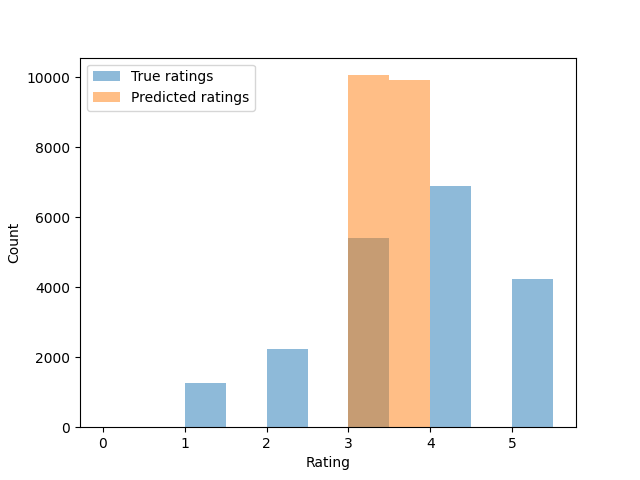
\includegraphics[scale=1]{figures/fig_1.png}
		\caption{Distribution of true and predicted ratings}
	\end{figure} 
	
	\begin{figure}[H]
		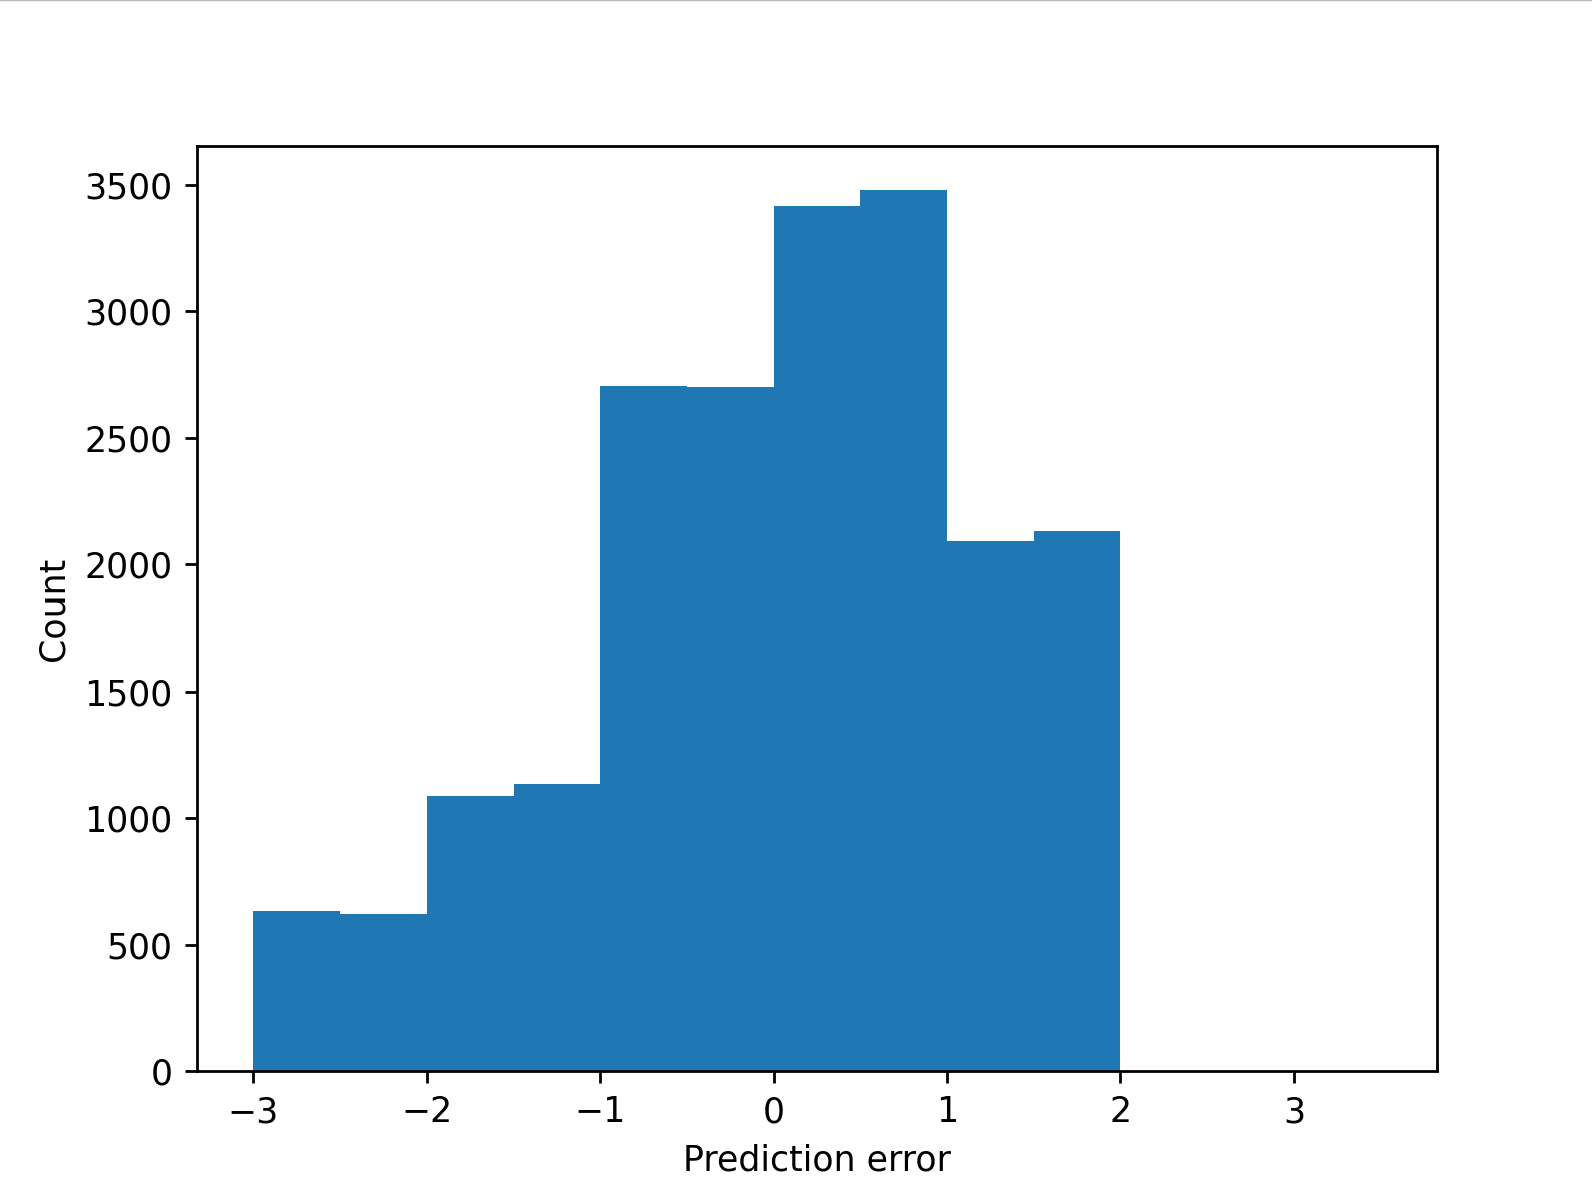
\includegraphics[scale=1]{figures/fig_2.png}
		\caption{Distribution of prediction errors}
	\end{figure} 
	
	\begin{figure}[H]
		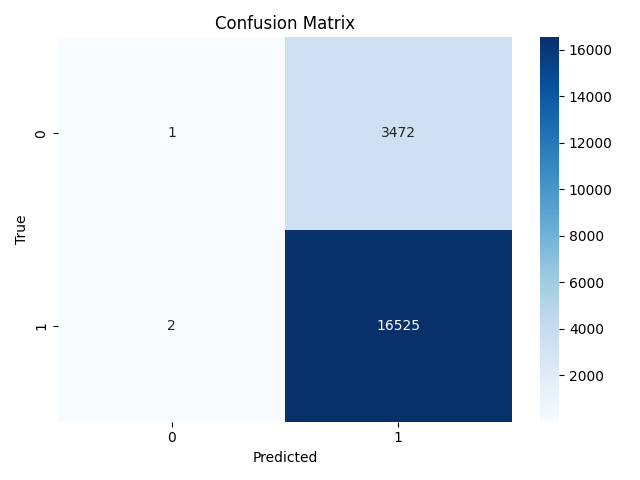
\includegraphics[scale=1]{figures/fig_3.png}
		\caption{Confusion Matrix}
	\end{figure} 
	
	Histograms of true and predicted ratings as well as prediction errors offer a visual representation of the model's predictive performance.
	These plots can reveal patterns in the distribution of ratings and errors, providing additional insights beyond numerical metrics. For example, on the plots we can clearly see that the model greatly favours predcting movie ratings between 3 and 4, avoiding the real distribution of ratings, and classifying almost all movies as favorable to be watched by any user.\\
	
	A confusion matrix provides a more detailed breakdown of the model's performance, showing true positives, true negatives, false positives, and false negatives.
	It helps in understanding where the model is making errors and provides insights into its strengths and weaknesses. In our case, histogram once again shows that model almost always predicts that the movie should be watched by a user, as there are no true negatives and there are no false negatives in the model predictions. \\
	
	After the plots, the evaluation script also writes down top 5 best movies for each user in the top5\_recommendations.txt file.
	
	The final results of the evaluation matrix are given below:
	\begin{table}[ht]
		\centering
		\begin{tabular}{|c|c|c|c|}
			\hline
			\textbf{RMSE} & \textbf{Precision} & \textbf{Recall} & \textbf{F1 score} \\
			\hline
			1.132 1 & 55.609\% & 100\% & 71.473\% \\
			\hline
		\end{tabular}
		\caption{Final Results}
		\label{tab:mytable}
	\end{table}
	
	Based on these results, we can make the following conclusions on the model performance:
	\begin{itemize}
		\item \textbf{Root Mean Square Error (RMSE)} - The RMSE value is 1.1321, indicating the average prediction error in the model. Lower RMSE values are generally better, and this value suggests that, on average, the model's predicted ratings deviate by approximately 1.13 from the actual ratings.
		\item \textbf{Precision} - The precision of 55.609\% suggests that when the model predicts a positive rating, it is correct approximately 55.6\% of the time. This metric is relevant in the context of positive ratings (e.g., high-quality recommendations), and we can see that many of the positive predictions made by the model are wrong, so it fails to capture the negatives.
		\item \textbf{Recall} - A recall of 100\% indicates that the model successfully identified all actual positive instances. In the context of a recommendation system, this means capturing all relevant movies that a user would like.
		\item \textbf{F1 Score} - The F1 score is the harmonic mean of precision and recall, providing a balanced measure of a model's performance. The F1 score of 71.473\% suggests a reasonable trade-off between precision and recall. A higher F1 score indicates a better balance between precision and recall.
	\end{itemize}
	
	To conclude, while our model captures all positive values, its performance is doubtful due to it almost never correctly identifying negative movies for various users.
	
	\begin{thebibliography}{99}
		\bibitem{main} https://github.com/MiladGhorbaniG/GNN-for-Recommendation-System/tree/main
	\end{thebibliography}
	
\end{document}



